% Created by tikzDevice version 0.10.1 on 2017-11-19 19:18:23
% !TEX encoding = UTF-8 Unicode
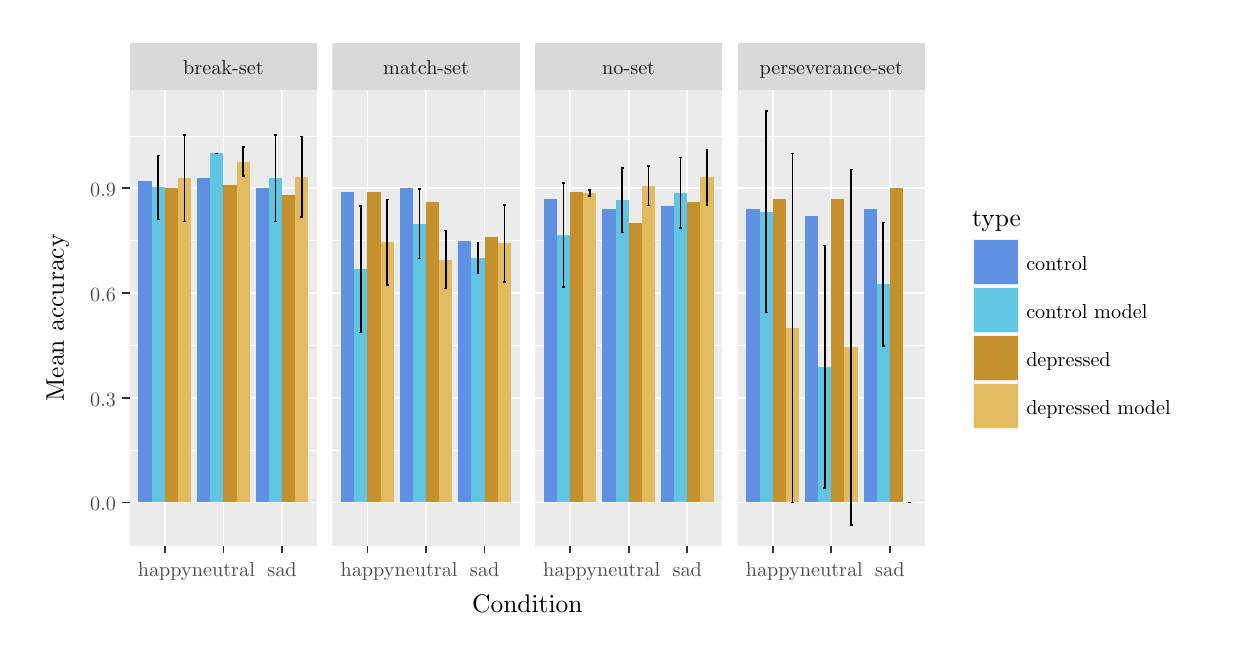
\begin{tikzpicture}[x=1pt,y=1pt]
\definecolor{fillColor}{RGB}{255,255,255}
\path[use as bounding box,fill=fillColor,fill opacity=0.00] (0,0) rectangle (433.62,216.81);
\begin{scope}
\path[clip] (  0.00,  0.00) rectangle (433.62,216.81);
\definecolor{drawColor}{RGB}{255,255,255}
\definecolor{fillColor}{RGB}{255,255,255}

\path[draw=drawColor,line width= 0.6pt,line join=round,line cap=round,fill=fillColor] (  0.00,  0.00) rectangle (433.62,216.81);
\end{scope}
\begin{scope}
\path[clip] ( 36.87, 29.59) rectangle (104.59,194.25);
\definecolor{fillColor}{gray}{0.92}

\path[fill=fillColor] ( 36.87, 29.59) rectangle (104.59,194.25);
\definecolor{drawColor}{RGB}{255,255,255}

\path[draw=drawColor,line width= 0.3pt,line join=round] ( 36.87, 64.16) --
	(104.59, 64.16);

\path[draw=drawColor,line width= 0.3pt,line join=round] ( 36.87,102.00) --
	(104.59,102.00);

\path[draw=drawColor,line width= 0.3pt,line join=round] ( 36.87,139.84) --
	(104.59,139.84);

\path[draw=drawColor,line width= 0.3pt,line join=round] ( 36.87,177.68) --
	(104.59,177.68);

\path[draw=drawColor,line width= 0.6pt,line join=round] ( 36.87, 45.24) --
	(104.59, 45.24);

\path[draw=drawColor,line width= 0.6pt,line join=round] ( 36.87, 83.08) --
	(104.59, 83.08);

\path[draw=drawColor,line width= 0.6pt,line join=round] ( 36.87,120.92) --
	(104.59,120.92);

\path[draw=drawColor,line width= 0.6pt,line join=round] ( 36.87,158.76) --
	(104.59,158.76);

\path[draw=drawColor,line width= 0.6pt,line join=round] ( 49.56, 29.59) --
	( 49.56,194.25);

\path[draw=drawColor,line width= 0.6pt,line join=round] ( 70.73, 29.59) --
	( 70.73,194.25);

\path[draw=drawColor,line width= 0.6pt,line join=round] ( 91.89, 29.59) --
	( 91.89,194.25);
\definecolor{fillColor}{RGB}{226,186,95}

\path[fill=fillColor] ( 54.33, 45.24) rectangle ( 59.09,162.36);
\definecolor{fillColor}{RGB}{196,145,45}

\path[fill=fillColor] ( 49.56, 45.24) rectangle ( 54.33,158.76);
\definecolor{fillColor}{RGB}{95,197,226}

\path[fill=fillColor] ( 44.80, 45.24) rectangle ( 49.56,159.06);
\definecolor{fillColor}{RGB}{95,145,226}

\path[fill=fillColor] ( 40.04, 45.24) rectangle ( 44.80,161.28);
\definecolor{fillColor}{RGB}{226,186,95}

\path[fill=fillColor] ( 75.49, 45.24) rectangle ( 80.25,168.37);
\definecolor{fillColor}{RGB}{196,145,45}

\path[fill=fillColor] ( 70.73, 45.24) rectangle ( 75.49,160.02);
\definecolor{fillColor}{RGB}{95,197,226}

\path[fill=fillColor] ( 65.97, 45.24) rectangle ( 70.73,171.37);
\definecolor{fillColor}{RGB}{95,145,226}

\path[fill=fillColor] ( 61.20, 45.24) rectangle ( 65.97,162.55);
\definecolor{fillColor}{RGB}{226,186,95}

\path[fill=fillColor] ( 96.65, 45.24) rectangle (101.41,162.97);
\definecolor{fillColor}{RGB}{196,145,45}

\path[fill=fillColor] ( 91.89, 45.24) rectangle ( 96.65,156.24);
\definecolor{fillColor}{RGB}{95,197,226}

\path[fill=fillColor] ( 87.13, 45.24) rectangle ( 91.89,162.36);
\definecolor{fillColor}{RGB}{95,145,226}

\path[fill=fillColor] ( 82.37, 45.24) rectangle ( 87.13,158.76);
\definecolor{drawColor}{RGB}{0,0,0}

\path[draw=drawColor,line width= 0.6pt,line join=round] ( 56.18,177.97) --
	( 57.24,177.97);

\path[draw=drawColor,line width= 0.6pt,line join=round] ( 56.71,177.97) --
	( 56.71,146.76);

\path[draw=drawColor,line width= 0.6pt,line join=round] ( 56.18,146.76) --
	( 57.24,146.76);

\path[draw=drawColor,line width= 0.6pt,line join=round] ( 46.65,170.62) --
	( 47.71,170.62);

\path[draw=drawColor,line width= 0.6pt,line join=round] ( 47.18,170.62) --
	( 47.18,147.50);

\path[draw=drawColor,line width= 0.6pt,line join=round] ( 46.65,147.50) --
	( 47.71,147.50);

\path[draw=drawColor,line width= 0.6pt,line join=round] ( 77.34,173.57) --
	( 78.40,173.57);

\path[draw=drawColor,line width= 0.6pt,line join=round] ( 77.87,173.57) --
	( 77.87,163.17);

\path[draw=drawColor,line width= 0.6pt,line join=round] ( 77.34,163.17) --
	( 78.40,163.17);

\path[draw=drawColor,line width= 0.6pt,line join=round] ( 67.82,171.37) --
	( 68.88,171.37);

\path[draw=drawColor,line width= 0.6pt,line join=round] ( 68.35,171.37) --
	( 68.35,171.37);

\path[draw=drawColor,line width= 0.6pt,line join=round] ( 67.82,171.37) --
	( 68.88,171.37);

\path[draw=drawColor,line width= 0.6pt,line join=round] ( 98.50,177.53) --
	( 99.56,177.53);

\path[draw=drawColor,line width= 0.6pt,line join=round] ( 99.03,177.53) --
	( 99.03,148.40);

\path[draw=drawColor,line width= 0.6pt,line join=round] ( 98.50,148.40) --
	( 99.56,148.40);

\path[draw=drawColor,line width= 0.6pt,line join=round] ( 88.98,177.97) --
	( 90.04,177.97);

\path[draw=drawColor,line width= 0.6pt,line join=round] ( 89.51,177.97) --
	( 89.51,146.76);

\path[draw=drawColor,line width= 0.6pt,line join=round] ( 88.98,146.76) --
	( 90.04,146.76);
\end{scope}
\begin{scope}
\path[clip] (110.09, 29.59) rectangle (177.81,194.25);
\definecolor{fillColor}{gray}{0.92}

\path[fill=fillColor] (110.09, 29.59) rectangle (177.81,194.25);
\definecolor{drawColor}{RGB}{255,255,255}

\path[draw=drawColor,line width= 0.3pt,line join=round] (110.09, 64.16) --
	(177.81, 64.16);

\path[draw=drawColor,line width= 0.3pt,line join=round] (110.09,102.00) --
	(177.81,102.00);

\path[draw=drawColor,line width= 0.3pt,line join=round] (110.09,139.84) --
	(177.81,139.84);

\path[draw=drawColor,line width= 0.3pt,line join=round] (110.09,177.68) --
	(177.81,177.68);

\path[draw=drawColor,line width= 0.6pt,line join=round] (110.09, 45.24) --
	(177.81, 45.24);

\path[draw=drawColor,line width= 0.6pt,line join=round] (110.09, 83.08) --
	(177.81, 83.08);

\path[draw=drawColor,line width= 0.6pt,line join=round] (110.09,120.92) --
	(177.81,120.92);

\path[draw=drawColor,line width= 0.6pt,line join=round] (110.09,158.76) --
	(177.81,158.76);

\path[draw=drawColor,line width= 0.6pt,line join=round] (122.79, 29.59) --
	(122.79,194.25);

\path[draw=drawColor,line width= 0.6pt,line join=round] (143.95, 29.59) --
	(143.95,194.25);

\path[draw=drawColor,line width= 0.6pt,line join=round] (165.11, 29.59) --
	(165.11,194.25);
\definecolor{fillColor}{RGB}{226,186,95}

\path[fill=fillColor] (127.55, 45.24) rectangle (132.31,139.30);
\definecolor{fillColor}{RGB}{196,145,45}

\path[fill=fillColor] (122.79, 45.24) rectangle (127.55,157.50);
\definecolor{fillColor}{RGB}{95,197,226}

\path[fill=fillColor] (118.02, 45.24) rectangle (122.79,129.51);
\definecolor{fillColor}{RGB}{95,145,226}

\path[fill=fillColor] (113.26, 45.24) rectangle (118.02,157.50);
\definecolor{fillColor}{RGB}{226,186,95}

\path[fill=fillColor] (148.71, 45.24) rectangle (153.47,132.98);
\definecolor{fillColor}{RGB}{196,145,45}

\path[fill=fillColor] (143.95, 45.24) rectangle (148.71,153.72);
\definecolor{fillColor}{RGB}{95,197,226}

\path[fill=fillColor] (139.19, 45.24) rectangle (143.95,146.02);
\definecolor{fillColor}{RGB}{95,145,226}

\path[fill=fillColor] (134.43, 45.24) rectangle (139.19,158.76);
\definecolor{fillColor}{RGB}{226,186,95}

\path[fill=fillColor] (169.87, 45.24) rectangle (174.64,138.87);
\definecolor{fillColor}{RGB}{196,145,45}

\path[fill=fillColor] (165.11, 45.24) rectangle (169.87,141.10);
\definecolor{fillColor}{RGB}{95,197,226}

\path[fill=fillColor] (160.35, 45.24) rectangle (165.11,133.71);
\definecolor{fillColor}{RGB}{95,145,226}

\path[fill=fillColor] (155.59, 45.24) rectangle (160.35,139.84);
\definecolor{drawColor}{RGB}{0,0,0}

\path[draw=drawColor,line width= 0.6pt,line join=round] (129.40,154.69) --
	(130.46,154.69);

\path[draw=drawColor,line width= 0.6pt,line join=round] (129.93,154.69) --
	(129.93,123.92);

\path[draw=drawColor,line width= 0.6pt,line join=round] (129.40,123.92) --
	(130.46,123.92);

\path[draw=drawColor,line width= 0.6pt,line join=round] (119.88,152.35) --
	(120.93,152.35);

\path[draw=drawColor,line width= 0.6pt,line join=round] (120.40,152.35) --
	(120.40,106.67);

\path[draw=drawColor,line width= 0.6pt,line join=round] (119.88,106.67) --
	(120.93,106.67);

\path[draw=drawColor,line width= 0.6pt,line join=round] (150.56,143.46) --
	(151.62,143.46);

\path[draw=drawColor,line width= 0.6pt,line join=round] (151.09,143.46) --
	(151.09,122.50);

\path[draw=drawColor,line width= 0.6pt,line join=round] (150.56,122.50) --
	(151.62,122.50);

\path[draw=drawColor,line width= 0.6pt,line join=round] (141.04,158.63) --
	(142.10,158.63);

\path[draw=drawColor,line width= 0.6pt,line join=round] (141.57,158.63) --
	(141.57,133.42);

\path[draw=drawColor,line width= 0.6pt,line join=round] (141.04,133.42) --
	(142.10,133.42);

\path[draw=drawColor,line width= 0.6pt,line join=round] (171.73,152.83) --
	(172.78,152.83);

\path[draw=drawColor,line width= 0.6pt,line join=round] (172.25,152.83) --
	(172.25,124.91);

\path[draw=drawColor,line width= 0.6pt,line join=round] (171.73,124.91) --
	(172.78,124.91);

\path[draw=drawColor,line width= 0.6pt,line join=round] (162.20,139.18) --
	(163.26,139.18);

\path[draw=drawColor,line width= 0.6pt,line join=round] (162.73,139.18) --
	(162.73,128.24);

\path[draw=drawColor,line width= 0.6pt,line join=round] (162.20,128.24) --
	(163.26,128.24);
\end{scope}
\begin{scope}
\path[clip] (183.31, 29.59) rectangle (251.03,194.25);
\definecolor{fillColor}{gray}{0.92}

\path[fill=fillColor] (183.31, 29.59) rectangle (251.03,194.25);
\definecolor{drawColor}{RGB}{255,255,255}

\path[draw=drawColor,line width= 0.3pt,line join=round] (183.31, 64.16) --
	(251.03, 64.16);

\path[draw=drawColor,line width= 0.3pt,line join=round] (183.31,102.00) --
	(251.03,102.00);

\path[draw=drawColor,line width= 0.3pt,line join=round] (183.31,139.84) --
	(251.03,139.84);

\path[draw=drawColor,line width= 0.3pt,line join=round] (183.31,177.68) --
	(251.03,177.68);

\path[draw=drawColor,line width= 0.6pt,line join=round] (183.31, 45.24) --
	(251.03, 45.24);

\path[draw=drawColor,line width= 0.6pt,line join=round] (183.31, 83.08) --
	(251.03, 83.08);

\path[draw=drawColor,line width= 0.6pt,line join=round] (183.31,120.92) --
	(251.03,120.92);

\path[draw=drawColor,line width= 0.6pt,line join=round] (183.31,158.76) --
	(251.03,158.76);

\path[draw=drawColor,line width= 0.6pt,line join=round] (196.01, 29.59) --
	(196.01,194.25);

\path[draw=drawColor,line width= 0.6pt,line join=round] (217.17, 29.59) --
	(217.17,194.25);

\path[draw=drawColor,line width= 0.6pt,line join=round] (238.33, 29.59) --
	(238.33,194.25);
\definecolor{fillColor}{RGB}{226,186,95}

\path[fill=fillColor] (200.77, 45.24) rectangle (205.53,157.03);
\definecolor{fillColor}{RGB}{196,145,45}

\path[fill=fillColor] (196.01, 45.24) rectangle (200.77,157.50);
\definecolor{fillColor}{RGB}{95,197,226}

\path[fill=fillColor] (191.25, 45.24) rectangle (196.01,141.86);
\definecolor{fillColor}{RGB}{95,145,226}

\path[fill=fillColor] (186.48, 45.24) rectangle (191.25,154.98);
\definecolor{fillColor}{RGB}{226,186,95}

\path[fill=fillColor] (221.93, 45.24) rectangle (226.69,159.72);
\definecolor{fillColor}{RGB}{196,145,45}

\path[fill=fillColor] (217.17, 45.24) rectangle (221.93,146.15);
\definecolor{fillColor}{RGB}{95,197,226}

\path[fill=fillColor] (212.41, 45.24) rectangle (217.17,154.41);
\definecolor{fillColor}{RGB}{95,145,226}

\path[fill=fillColor] (207.65, 45.24) rectangle (212.41,151.19);
\definecolor{fillColor}{RGB}{226,186,95}

\path[fill=fillColor] (243.10, 45.24) rectangle (247.86,162.69);
\definecolor{fillColor}{RGB}{196,145,45}

\path[fill=fillColor] (238.33, 45.24) rectangle (243.10,153.72);
\definecolor{fillColor}{RGB}{95,197,226}

\path[fill=fillColor] (233.57, 45.24) rectangle (238.33,157.20);
\definecolor{fillColor}{RGB}{95,145,226}

\path[fill=fillColor] (228.81, 45.24) rectangle (233.57,152.45);
\definecolor{drawColor}{RGB}{0,0,0}

\path[draw=drawColor,line width= 0.6pt,line join=round] (202.62,158.16) --
	(203.68,158.16);

\path[draw=drawColor,line width= 0.6pt,line join=round] (203.15,158.16) --
	(203.15,155.90);

\path[draw=drawColor,line width= 0.6pt,line join=round] (202.62,155.90) --
	(203.68,155.90);

\path[draw=drawColor,line width= 0.6pt,line join=round] (193.10,160.70) --
	(194.16,160.70);

\path[draw=drawColor,line width= 0.6pt,line join=round] (193.63,160.70) --
	(193.63,123.02);

\path[draw=drawColor,line width= 0.6pt,line join=round] (193.10,123.02) --
	(194.16,123.02);

\path[draw=drawColor,line width= 0.6pt,line join=round] (223.78,166.93) --
	(224.84,166.93);

\path[draw=drawColor,line width= 0.6pt,line join=round] (224.31,166.93) --
	(224.31,152.51);

\path[draw=drawColor,line width= 0.6pt,line join=round] (223.78,152.51) --
	(224.84,152.51);

\path[draw=drawColor,line width= 0.6pt,line join=round] (214.26,166.01) --
	(215.32,166.01);

\path[draw=drawColor,line width= 0.6pt,line join=round] (214.79,166.01) --
	(214.79,142.82);

\path[draw=drawColor,line width= 0.6pt,line join=round] (214.26,142.82) --
	(215.32,142.82);

\path[draw=drawColor,line width= 0.6pt,line join=round] (244.95,172.56) --
	(246.01,172.56);

\path[draw=drawColor,line width= 0.6pt,line join=round] (245.48,172.56) --
	(245.48,152.83);

\path[draw=drawColor,line width= 0.6pt,line join=round] (244.95,152.83) --
	(246.01,152.83);

\path[draw=drawColor,line width= 0.6pt,line join=round] (235.42,169.92) --
	(236.48,169.92);

\path[draw=drawColor,line width= 0.6pt,line join=round] (235.95,169.92) --
	(235.95,144.48);

\path[draw=drawColor,line width= 0.6pt,line join=round] (235.42,144.48) --
	(236.48,144.48);
\end{scope}
\begin{scope}
\path[clip] (256.53, 29.59) rectangle (324.25,194.25);
\definecolor{fillColor}{gray}{0.92}

\path[fill=fillColor] (256.53, 29.59) rectangle (324.25,194.25);
\definecolor{drawColor}{RGB}{255,255,255}

\path[draw=drawColor,line width= 0.3pt,line join=round] (256.53, 64.16) --
	(324.25, 64.16);

\path[draw=drawColor,line width= 0.3pt,line join=round] (256.53,102.00) --
	(324.25,102.00);

\path[draw=drawColor,line width= 0.3pt,line join=round] (256.53,139.84) --
	(324.25,139.84);

\path[draw=drawColor,line width= 0.3pt,line join=round] (256.53,177.68) --
	(324.25,177.68);

\path[draw=drawColor,line width= 0.6pt,line join=round] (256.53, 45.24) --
	(324.25, 45.24);

\path[draw=drawColor,line width= 0.6pt,line join=round] (256.53, 83.08) --
	(324.25, 83.08);

\path[draw=drawColor,line width= 0.6pt,line join=round] (256.53,120.92) --
	(324.25,120.92);

\path[draw=drawColor,line width= 0.6pt,line join=round] (256.53,158.76) --
	(324.25,158.76);

\path[draw=drawColor,line width= 0.6pt,line join=round] (269.23, 29.59) --
	(269.23,194.25);

\path[draw=drawColor,line width= 0.6pt,line join=round] (290.39, 29.59) --
	(290.39,194.25);

\path[draw=drawColor,line width= 0.6pt,line join=round] (311.56, 29.59) --
	(311.56,194.25);
\definecolor{fillColor}{RGB}{226,186,95}

\path[fill=fillColor] (273.99, 45.24) rectangle (278.75,108.31);
\definecolor{fillColor}{RGB}{196,145,45}

\path[fill=fillColor] (269.23, 45.24) rectangle (273.99,154.98);
\definecolor{fillColor}{RGB}{95,197,226}

\path[fill=fillColor] (264.47, 45.24) rectangle (269.23,150.35);
\definecolor{fillColor}{RGB}{95,145,226}

\path[fill=fillColor] (259.71, 45.24) rectangle (264.47,151.19);
\definecolor{fillColor}{RGB}{226,186,95}

\path[fill=fillColor] (295.15, 45.24) rectangle (299.92,101.30);
\definecolor{fillColor}{RGB}{196,145,45}

\path[fill=fillColor] (290.39, 45.24) rectangle (295.15,154.98);
\definecolor{fillColor}{RGB}{95,197,226}

\path[fill=fillColor] (285.63, 45.24) rectangle (290.39, 94.29);
\definecolor{fillColor}{RGB}{95,145,226}

\path[fill=fillColor] (280.87, 45.24) rectangle (285.63,148.67);
\definecolor{fillColor}{RGB}{226,186,95}

\path[fill=fillColor] (316.32, 45.24) rectangle (321.08, 45.24);
\definecolor{fillColor}{RGB}{196,145,45}

\path[fill=fillColor] (311.56, 45.24) rectangle (316.32,158.76);
\definecolor{fillColor}{RGB}{95,197,226}

\path[fill=fillColor] (306.79, 45.24) rectangle (311.56,124.07);
\definecolor{fillColor}{RGB}{95,145,226}

\path[fill=fillColor] (302.03, 45.24) rectangle (306.79,151.19);
\definecolor{drawColor}{RGB}{0,0,0}

\path[draw=drawColor,line width= 0.6pt,line join=round] (275.84,171.37) --
	(276.90,171.37);

\path[draw=drawColor,line width= 0.6pt,line join=round] (276.37,171.37) --
	(276.37, 45.24);

\path[draw=drawColor,line width= 0.6pt,line join=round] (275.84, 45.24) --
	(276.90, 45.24);

\path[draw=drawColor,line width= 0.6pt,line join=round] (266.32,186.76) --
	(267.38,186.76);

\path[draw=drawColor,line width= 0.6pt,line join=round] (266.85,186.76) --
	(266.85,113.94);

\path[draw=drawColor,line width= 0.6pt,line join=round] (266.32,113.94) --
	(267.38,113.94);

\path[draw=drawColor,line width= 0.6pt,line join=round] (297.01,165.52) --
	(298.06,165.52);

\path[draw=drawColor,line width= 0.6pt,line join=round] (297.53,165.52) --
	(297.53, 37.07);

\path[draw=drawColor,line width= 0.6pt,line join=round] (297.01, 37.07) --
	(298.06, 37.07);

\path[draw=drawColor,line width= 0.6pt,line join=round] (287.48,138.05) --
	(288.54,138.05);

\path[draw=drawColor,line width= 0.6pt,line join=round] (288.01,138.05) --
	(288.01, 50.53);

\path[draw=drawColor,line width= 0.6pt,line join=round] (287.48, 50.53) --
	(288.54, 50.53);

\path[draw=drawColor,line width= 0.6pt,line join=round] (318.17, 45.24) --
	(319.23, 45.24);

\path[draw=drawColor,line width= 0.6pt,line join=round] (318.70, 45.24) --
	(318.70, 45.24);

\path[draw=drawColor,line width= 0.6pt,line join=round] (318.17, 45.24) --
	(319.23, 45.24);

\path[draw=drawColor,line width= 0.6pt,line join=round] (308.65,146.37) --
	(309.70,146.37);

\path[draw=drawColor,line width= 0.6pt,line join=round] (309.17,146.37) --
	(309.17,101.77);

\path[draw=drawColor,line width= 0.6pt,line join=round] (308.65,101.77) --
	(309.70,101.77);
\end{scope}
\begin{scope}
\path[clip] ( 36.87,194.25) rectangle (104.59,211.31);
\definecolor{fillColor}{gray}{0.85}

\path[fill=fillColor] ( 36.87,194.25) rectangle (104.59,211.31);
\definecolor{drawColor}{gray}{0.10}

\node[text=drawColor,anchor=base,inner sep=0pt, outer sep=0pt, scale=  0.73] at ( 70.73,199.75) {break-set};
\end{scope}
\begin{scope}
\path[clip] (110.09,194.25) rectangle (177.81,211.31);
\definecolor{fillColor}{gray}{0.85}

\path[fill=fillColor] (110.09,194.25) rectangle (177.81,211.31);
\definecolor{drawColor}{gray}{0.10}

\node[text=drawColor,anchor=base,inner sep=0pt, outer sep=0pt, scale=  0.73] at (143.95,199.75) {match-set};
\end{scope}
\begin{scope}
\path[clip] (183.31,194.25) rectangle (251.03,211.31);
\definecolor{fillColor}{gray}{0.85}

\path[fill=fillColor] (183.31,194.25) rectangle (251.03,211.31);
\definecolor{drawColor}{gray}{0.10}

\node[text=drawColor,anchor=base,inner sep=0pt, outer sep=0pt, scale=  0.73] at (217.17,199.75) {no-set};
\end{scope}
\begin{scope}
\path[clip] (256.53,194.25) rectangle (324.25,211.31);
\definecolor{fillColor}{gray}{0.85}

\path[fill=fillColor] (256.53,194.25) rectangle (324.25,211.31);
\definecolor{drawColor}{gray}{0.10}

\node[text=drawColor,anchor=base,inner sep=0pt, outer sep=0pt, scale=  0.73] at (290.39,199.75) {perseverance-set};
\end{scope}
\begin{scope}
\path[clip] (  0.00,  0.00) rectangle (433.62,216.81);
\definecolor{drawColor}{gray}{0.20}

\path[draw=drawColor,line width= 0.6pt,line join=round] ( 49.56, 26.84) --
	( 49.56, 29.59);

\path[draw=drawColor,line width= 0.6pt,line join=round] ( 70.73, 26.84) --
	( 70.73, 29.59);

\path[draw=drawColor,line width= 0.6pt,line join=round] ( 91.89, 26.84) --
	( 91.89, 29.59);
\end{scope}
\begin{scope}
\path[clip] (  0.00,  0.00) rectangle (433.62,216.81);
\definecolor{drawColor}{gray}{0.30}

\node[text=drawColor,anchor=base,inner sep=0pt, outer sep=0pt, scale=  0.73] at ( 49.56, 18.58) {happy};

\node[text=drawColor,anchor=base,inner sep=0pt, outer sep=0pt, scale=  0.73] at ( 70.73, 18.58) {neutral};

\node[text=drawColor,anchor=base,inner sep=0pt, outer sep=0pt, scale=  0.73] at ( 91.89, 18.58) {sad};
\end{scope}
\begin{scope}
\path[clip] (  0.00,  0.00) rectangle (433.62,216.81);
\definecolor{drawColor}{gray}{0.20}

\path[draw=drawColor,line width= 0.6pt,line join=round] (122.79, 26.84) --
	(122.79, 29.59);

\path[draw=drawColor,line width= 0.6pt,line join=round] (143.95, 26.84) --
	(143.95, 29.59);

\path[draw=drawColor,line width= 0.6pt,line join=round] (165.11, 26.84) --
	(165.11, 29.59);
\end{scope}
\begin{scope}
\path[clip] (  0.00,  0.00) rectangle (433.62,216.81);
\definecolor{drawColor}{gray}{0.30}

\node[text=drawColor,anchor=base,inner sep=0pt, outer sep=0pt, scale=  0.73] at (122.79, 18.58) {happy};

\node[text=drawColor,anchor=base,inner sep=0pt, outer sep=0pt, scale=  0.73] at (143.95, 18.58) {neutral};

\node[text=drawColor,anchor=base,inner sep=0pt, outer sep=0pt, scale=  0.73] at (165.11, 18.58) {sad};
\end{scope}
\begin{scope}
\path[clip] (  0.00,  0.00) rectangle (433.62,216.81);
\definecolor{drawColor}{gray}{0.20}

\path[draw=drawColor,line width= 0.6pt,line join=round] (196.01, 26.84) --
	(196.01, 29.59);

\path[draw=drawColor,line width= 0.6pt,line join=round] (217.17, 26.84) --
	(217.17, 29.59);

\path[draw=drawColor,line width= 0.6pt,line join=round] (238.33, 26.84) --
	(238.33, 29.59);
\end{scope}
\begin{scope}
\path[clip] (  0.00,  0.00) rectangle (433.62,216.81);
\definecolor{drawColor}{gray}{0.30}

\node[text=drawColor,anchor=base,inner sep=0pt, outer sep=0pt, scale=  0.73] at (196.01, 18.58) {happy};

\node[text=drawColor,anchor=base,inner sep=0pt, outer sep=0pt, scale=  0.73] at (217.17, 18.58) {neutral};

\node[text=drawColor,anchor=base,inner sep=0pt, outer sep=0pt, scale=  0.73] at (238.33, 18.58) {sad};
\end{scope}
\begin{scope}
\path[clip] (  0.00,  0.00) rectangle (433.62,216.81);
\definecolor{drawColor}{gray}{0.20}

\path[draw=drawColor,line width= 0.6pt,line join=round] (269.23, 26.84) --
	(269.23, 29.59);

\path[draw=drawColor,line width= 0.6pt,line join=round] (290.39, 26.84) --
	(290.39, 29.59);

\path[draw=drawColor,line width= 0.6pt,line join=round] (311.56, 26.84) --
	(311.56, 29.59);
\end{scope}
\begin{scope}
\path[clip] (  0.00,  0.00) rectangle (433.62,216.81);
\definecolor{drawColor}{gray}{0.30}

\node[text=drawColor,anchor=base,inner sep=0pt, outer sep=0pt, scale=  0.73] at (269.23, 18.58) {happy};

\node[text=drawColor,anchor=base,inner sep=0pt, outer sep=0pt, scale=  0.73] at (290.39, 18.58) {neutral};

\node[text=drawColor,anchor=base,inner sep=0pt, outer sep=0pt, scale=  0.73] at (311.56, 18.58) {sad};
\end{scope}
\begin{scope}
\path[clip] (  0.00,  0.00) rectangle (433.62,216.81);
\definecolor{drawColor}{gray}{0.30}

\node[text=drawColor,anchor=base east,inner sep=0pt, outer sep=0pt, scale=  0.73] at ( 31.92, 42.21) {0.0};

\node[text=drawColor,anchor=base east,inner sep=0pt, outer sep=0pt, scale=  0.73] at ( 31.92, 80.05) {0.3};

\node[text=drawColor,anchor=base east,inner sep=0pt, outer sep=0pt, scale=  0.73] at ( 31.92,117.89) {0.6};

\node[text=drawColor,anchor=base east,inner sep=0pt, outer sep=0pt, scale=  0.73] at ( 31.92,155.73) {0.9};
\end{scope}
\begin{scope}
\path[clip] (  0.00,  0.00) rectangle (433.62,216.81);
\definecolor{drawColor}{gray}{0.20}

\path[draw=drawColor,line width= 0.6pt,line join=round] ( 34.12, 45.24) --
	( 36.87, 45.24);

\path[draw=drawColor,line width= 0.6pt,line join=round] ( 34.12, 83.08) --
	( 36.87, 83.08);

\path[draw=drawColor,line width= 0.6pt,line join=round] ( 34.12,120.92) --
	( 36.87,120.92);

\path[draw=drawColor,line width= 0.6pt,line join=round] ( 34.12,158.76) --
	( 36.87,158.76);
\end{scope}
\begin{scope}
\path[clip] (  0.00,  0.00) rectangle (433.62,216.81);
\definecolor{drawColor}{RGB}{0,0,0}

\node[text=drawColor,anchor=base,inner sep=0pt, outer sep=0pt, scale=  0.92] at (180.56,  5.50) {Condition};
\end{scope}
\begin{scope}
\path[clip] (  0.00,  0.00) rectangle (433.62,216.81);
\definecolor{drawColor}{RGB}{0,0,0}

\node[text=drawColor,rotate= 90.00,anchor=base,inner sep=0pt, outer sep=0pt, scale=  0.92] at ( 13.08,111.92) {Mean accuracy};
\end{scope}
\begin{scope}
\path[clip] (  0.00,  0.00) rectangle (433.62,216.81);
\definecolor{fillColor}{RGB}{255,255,255}

\path[fill=fillColor] (335.63, 65.58) rectangle (428.12,158.25);
\end{scope}
\begin{scope}
\path[clip] (  0.00,  0.00) rectangle (433.62,216.81);
\definecolor{drawColor}{RGB}{0,0,0}

\node[text=drawColor,anchor=base west,inner sep=0pt, outer sep=0pt, scale=  0.92] at (341.32,144.99) {type};
\end{scope}
\begin{scope}
\path[clip] (  0.00,  0.00) rectangle (433.62,216.81);
\definecolor{drawColor}{RGB}{255,255,255}
\definecolor{fillColor}{gray}{0.95}

\path[draw=drawColor,line width= 0.6pt,line join=round,line cap=round,fill=fillColor] (341.32,123.31) rectangle (358.67,140.65);
\end{scope}
\begin{scope}
\path[clip] (  0.00,  0.00) rectangle (433.62,216.81);
\definecolor{fillColor}{RGB}{95,145,226}

\path[fill=fillColor] (342.04,124.02) rectangle (357.96,139.94);
\end{scope}
\begin{scope}
\path[clip] (  0.00,  0.00) rectangle (433.62,216.81);
\definecolor{drawColor}{RGB}{255,255,255}
\definecolor{fillColor}{gray}{0.95}

\path[draw=drawColor,line width= 0.6pt,line join=round,line cap=round,fill=fillColor] (341.32,105.96) rectangle (358.67,123.31);
\end{scope}
\begin{scope}
\path[clip] (  0.00,  0.00) rectangle (433.62,216.81);
\definecolor{fillColor}{RGB}{95,197,226}

\path[fill=fillColor] (342.04,106.67) rectangle (357.96,122.60);
\end{scope}
\begin{scope}
\path[clip] (  0.00,  0.00) rectangle (433.62,216.81);
\definecolor{drawColor}{RGB}{255,255,255}
\definecolor{fillColor}{gray}{0.95}

\path[draw=drawColor,line width= 0.6pt,line join=round,line cap=round,fill=fillColor] (341.32, 88.62) rectangle (358.67,105.96);
\end{scope}
\begin{scope}
\path[clip] (  0.00,  0.00) rectangle (433.62,216.81);
\definecolor{fillColor}{RGB}{196,145,45}

\path[fill=fillColor] (342.04, 89.33) rectangle (357.96,105.25);
\end{scope}
\begin{scope}
\path[clip] (  0.00,  0.00) rectangle (433.62,216.81);
\definecolor{drawColor}{RGB}{255,255,255}
\definecolor{fillColor}{gray}{0.95}

\path[draw=drawColor,line width= 0.6pt,line join=round,line cap=round,fill=fillColor] (341.32, 71.27) rectangle (358.67, 88.62);
\end{scope}
\begin{scope}
\path[clip] (  0.00,  0.00) rectangle (433.62,216.81);
\definecolor{fillColor}{RGB}{226,186,95}

\path[fill=fillColor] (342.04, 71.98) rectangle (357.96, 87.91);
\end{scope}
\begin{scope}
\path[clip] (  0.00,  0.00) rectangle (433.62,216.81);
\definecolor{drawColor}{RGB}{0,0,0}

\node[text=drawColor,anchor=base west,inner sep=0pt, outer sep=0pt, scale=  0.73] at (360.84,128.95) {control};
\end{scope}
\begin{scope}
\path[clip] (  0.00,  0.00) rectangle (433.62,216.81);
\definecolor{drawColor}{RGB}{0,0,0}

\node[text=drawColor,anchor=base west,inner sep=0pt, outer sep=0pt, scale=  0.73] at (360.84,111.60) {control model};
\end{scope}
\begin{scope}
\path[clip] (  0.00,  0.00) rectangle (433.62,216.81);
\definecolor{drawColor}{RGB}{0,0,0}

\node[text=drawColor,anchor=base west,inner sep=0pt, outer sep=0pt, scale=  0.73] at (360.84, 94.26) {depressed};
\end{scope}
\begin{scope}
\path[clip] (  0.00,  0.00) rectangle (433.62,216.81);
\definecolor{drawColor}{RGB}{0,0,0}

\node[text=drawColor,anchor=base west,inner sep=0pt, outer sep=0pt, scale=  0.73] at (360.84, 76.91) {depressed model};
\end{scope}
\end{tikzpicture}
